% Fuente: Pauta del Auxiliar 10, «Repaso de programación entera — Cortes de Gomory».
{\color{MidnightBlue}
\begin{enumerate}
  \item
\begin{figure}
    \centering
    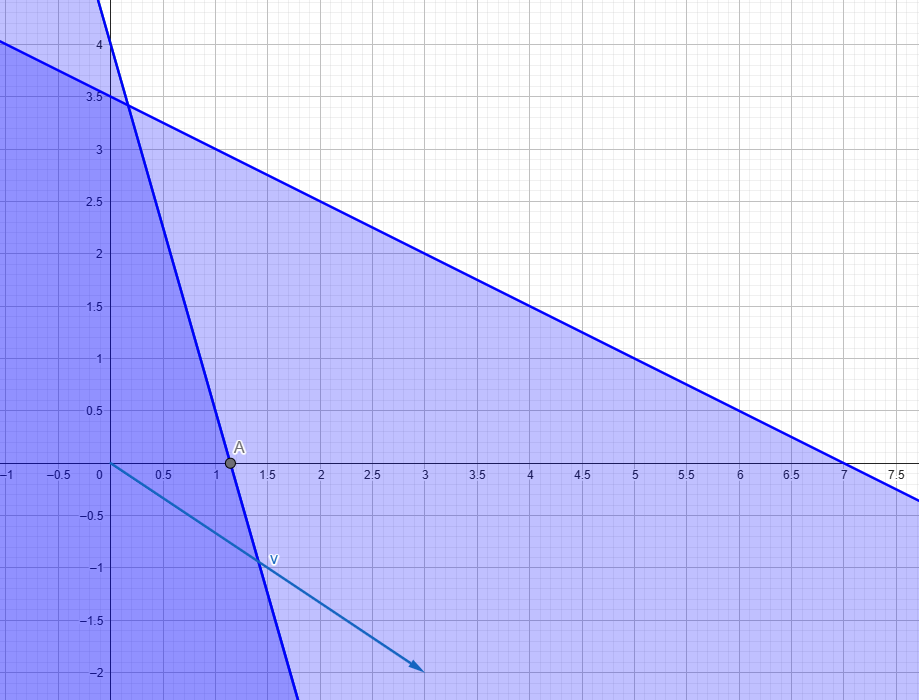
\includegraphics[width=0.8\linewidth]{img/ejercicios/Capitulo-5/ejercicio_5_4_solucion_gomory.png}
    \caption{Solución relajación lineal}
    \label{ex:5:4:fig:relajacion}
\end{figure}
    
El óptimo de la relajación se obtiene en
\[
(x_{1}^{*},x_{2}^{*}) = \Bigl(\tfrac{8}{7},0\Bigr),
\qquad
z^{*} = -3\cdot\tfrac{8}{7} + 2\cdot 0 = -\tfrac{24}{7}.
\]

Los puntos enteros factibles son:
\[
\{(0,0),(0,1),(0,2),(0,3),(1,0)\}.
\]

La envolvente convexa tiene vértices
\((0,0),(1,0),(0,3)\) y viene dada por
\[
x_{1}\ge0,\quad x_{2}\ge0,\quad 3x_{1}+x_{2}\le3.
\]

\begin{figure}
    \centering
    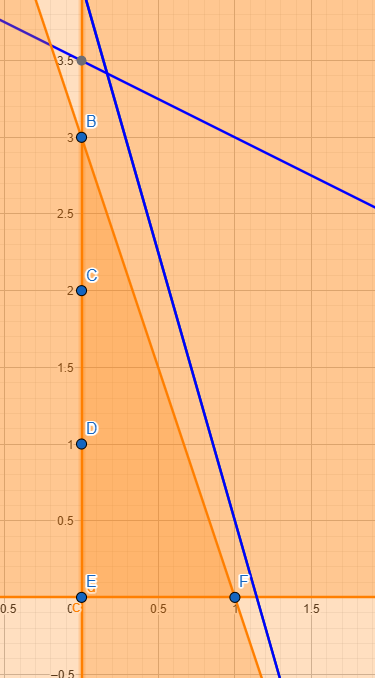
\includegraphics[width=0.5\linewidth]{img/ejercicios/Capitulo-5/ejercicio_5_4_envoltura_convexa.png}
    \caption{Envolvente convexa}
    \label{ex:5:4:fig:envoltura}
\end{figure}
  \item
Las matrices del problema relajado en formulación estándar son:
\[
A=\begin{pmatrix*}
7 & 2 & 1 & 0\\
1 & 2 & 0 & 1
\end{pmatrix*},\qquad
b=\begin{pmatrix}
8\\[0.3em]
7
\end{pmatrix},\qquad
B=\begin{pmatrix}
7 & 0\\
1 & 1
\end{pmatrix}
\]
El óptimo de la relajación lineal es
\[
(x_{1},x_{2},s_{1},s_{2})
=\Bigl(\tfrac{8}{7},\;0,\;0,\;\tfrac{41}{7}\Bigr),
\]
luego se realiza el corte sobre \(x_{1}\):
\begin{equation*}
x_{1}
\;+\;\bigl\lfloor\overline{a}_{12}\bigr\rfloor\,x_{2}
\;+\;\bigl\lfloor\overline{a}_{13}\bigr\rfloor\,s_{1}
\;\le\;\bigl\lfloor\overline{a}_{10}\bigr\rfloor
\end{equation*}
donde
\begin{align*}
\overline{a}_{12}
&=\Bigl(B^{-1}\begin{pmatrix}2\\2\end{pmatrix}\Bigr)_{1}
=\frac{2}{7},\\
\overline{a}_{13}
&=\Bigl(B^{-1}\begin{pmatrix}1\\0\end{pmatrix}\Bigr)_{1}
=\frac{1}{7},\\
\overline{a}_{10}
&=\Bigl(B^{-1}b\Bigr)_{1}
=\frac{8}{7}.
\end{align*}
De modo que el nuevo corte es:
\begin{equation*}
x_{1}\;\le\;1.
\end{equation*}
Añadiendo \(x_{1}\le1\) a la relajación original, el nuevo óptimo es
\[
(x_{1},x_{2}) = (1,0),\qquad z = -3,
\]
que ya es entero y coincide con la solución óptima del programa entero. 
\end{enumerate}
}
